%author akira treize
\documentclass[a4paper,12pt]{book}%document pour un papier a4 , police 12,type book
\usepackage[utf8]{inputenc}%type de codage
\usepackage{setspace}%pour utiliser onehalfspace ou autres
%\pagestyle{plain}
\usepackage[pdftex]{graphicx}%permet d'inserer des images
\usepackage{color}%utiliser les color dans latex
\usepackage[avantgarde]{quotchap}%style de pages chap en gris
\usepackage{fullpage}%utiliser tt la pages ou aulieu de la mise en forme par defaut de latex 
\usepackage{listings}%carre nume pour les codes ou lignes de commande
\usepackage{lettrine}
\usepackage{type1cm}%Font Shape Specifications generalment on va l'utiliser pour la 'taille de lettrine'
%\usepackage[T1]{fontenc}
\usepackage{wrapfig}

\setcounter{secnumdepth}{3}%pour la numérotation dans le corps du document
\setcounter{tocdepth}{3}%pour l'apparition dans la table des matières
 
\renewcommand{\baselinestretch}{1.5}%au lieu de one half space 
\renewcommand{\LettrineFontHook}{\color[gray]{0.5}}

\begin{document}
  \frontmatter%numerutation des pages sous forme de i 
  \tableofcontents%sommaire
  \listoffigures%liste des figure
%---------------------------------------------------------------------------------------------------------
% \begin{onehalfspace}
  \mainmatter%numerutation des pages en num arabe
  \chapter{General introduction}
\lettrine[lines=3]{T}{} he cloud computing "is a concept evolved relatively recently, but whose beginnings date back a few years, 
especially in the technology of grid computing, used for scientific computing.
\paragraph{}Cloud computing refers to the use of memory and computing capabilities of computers and servers around the world, 
and linked by a network, such as the Internet. 
Users of the cloud may well have considerable computing power and scalable.\par
\paragraph{}In our day cloud computing is used by almost all users: gmail, facebook, flikr, youtube and etc ... Because cloud computing is revolutionizing 
the whole computer system companies. Allowing both to reduce investment costs, 
improve working methods, this concept has the power to change corporate strategy.\par
\paragraph{}in 2012, one in three companies should use a cloud service. 
This is what the study says "Cloud Computing \& SaaS: Expectations and Prospects" conducted by the International Markess.\par
\paragraph{}But this miracle solution, have a big problem Security issues and Data Loss because Implementations that rely on the Internet 
as a means to improve operations are also prone to security problems, 
particularly from cybercriminals who are now looking to profit from attacking business entities.\par

\paragraph{}In our final project year we offer to create an android application that manages a cloud,
 by following this report will be divided into four chapters:
\begin{itemize}
 \item State of the Art
 \item Installing Nova
 \item Design phase
 \item Implementation and testing
\end{itemize}




  %author akira treize
\chapter{State Of The Art}
\lettrine[lines=3]{I}{} n this chapter we will see the various cloud solutions (eucalyptus, Open Nebula, Open Stack)
 offered on the Net as well as platforms for smart phones (IOS, Blackberry, Windows Phone, Android), 
but our choice will be based on the best solution accessible and available on documentations.
During our final year project, we will focus on free and open sources software and solutions to others alternative.
\paragraph{}In this chapter we present the cloud computing in general and the differing layer which composes and
our choice of cloud solution and platforms.\par

%%%%%%%%%%%%%%%%%%%%%%%%%%%%%%%%%%%%%%%%%%%%%%%%%%%%%%%%%%%%%%%%%%%%%%%%%%%%%%%%%%%%%%%%%%%%%%%%%%%%%%%%%%%%%%%%%%%%%%%%%%%%%%%%%%%
\newpage
\section{Cloud Computing}
\subsection{Introduction}
Cloud Computing  was a technical resource to handle (servers) rather than a product and to adapt quickly to changes in infrastructure load with complete
transparent to the administrator and users,whereby shared resources, software,
 and information are provided to computers and other devices as a metered service over a network (typically the Internet).

In the cloud, the customer is not afraid of the complexity of managing hardware behind its software environment.
\begin{figure}[!h]
 \center
 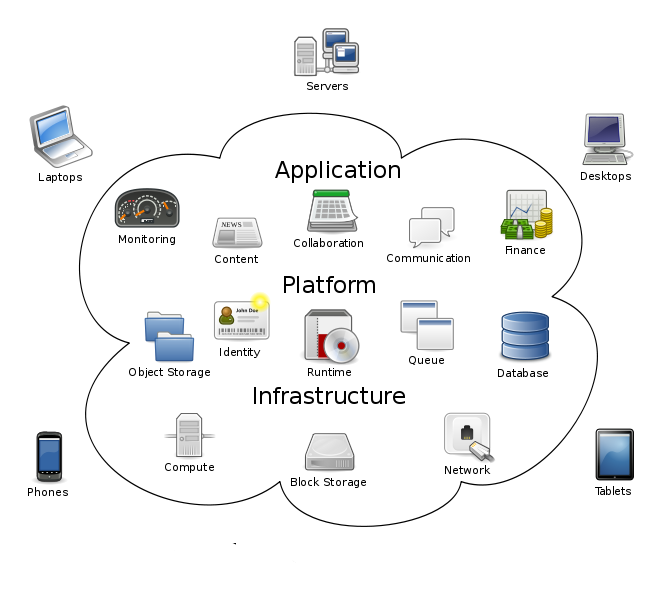
\includegraphics[width=8cm, height=7cm]{./images/Cloudcomputing.png}
 \caption{Cloud Computing}
\end{figure}



\subsection{the different layers on the cloud :}

Cloud computing is a concept:
\begin{itemize}
 \item Deport a remote infrastructure applications and data;
 \item Abstracting the management of infrastructure and material resources to customers.
\end{itemize}
 There was exactly four layers in the cloud classified by use:

\subsubsection{Infrastructure as a Service (IaaS):}

This layer is probably the most important because it rests on it as part of the other layers. It offers the possibility to rent, 
buy virtual machines, virtual servers on demand, but also storage.
Here is an example of the company offering IaaS: Amazon EC2 if you want to test, you can create an account and start an instance of type "micro" free for one year.
Otherwise, it is also possible to create its own layer IaaS, 
for this it is necessary to use a platform to implement and manage different virtual machines running in the IaaS layer, here are some open source platforms:

\begin {itemize}
 \item [•]Eucalyptus
 \item [•]OpenStack
 \item [•]OpenNebula
\end {itemize}

Eucalyptus is the platform used by Amazon EC2, OpenNebula is the recommended platform for Europe and developed by a Spanish company, 
OpenStack is a American platform developed by NASA.


\subsubsection{Platform as a Service (PaaS):}

This layer can be based directly on the previous one, it mainly concerns people making web development 
or web-oriented software. This means that developers can buy, rent a platform to develop their application in a language (Ruby, PHP, Java, ...)
 or through a particular framework.
The advantage is that there is no server to configure in-house, everything is ready and when the development is finished, the rented platform can be throw.
Here is one of the best known examples in the world of PaaS: Google App Engine


\subsubsection{Software as a Service (SaaS):}

This is undoubtedly the most famous layer and the most currently used. When you use Google Docs is the layer of SaaS Google services 
you use without knowing it! Or Drupal Services Garden, it's SaaS.
It becomes possible to deploy a website, a software without having to do installation, maintenance, etc ... 
You rent the software, it works and you can use it directly through your browser.
This layer can also be based on the previous layer and allow the developer to access the application that he has created.

% \subsection{Data as a Service (DaaS):} 
% \begin{onehalfspace}
% DaaS is a cousin of Software as a Service, is based on the concept that the data can be provided upon request to the user regardless of the distance between user and supplier data. 
% Enter data as a service (DaaS), by outsourcing data rather than software, enterprises can effectively have their cake and eat it. 
% Their data is maintained and served off-site, and independent software can plug into that data pool and use it in any number of ways. 
% This software can be custom-built, it can be a simple (and familiar) web form or Excel look-up, or it can of course be SaaS.
% Data as a service offers all the benefits of Software as a Service, but without the same restrictions.
% The online storage services are used to store data and documents without having to continually increase the number of servers or the size of SAN(Storage Area Network is a specialized network to contribute storage resources).
% The following services are based on cloud computing:
% \begin{itemize}
%  \item [•]Dropbox
%  \item [•]Amazon Simple Storage Service
%  \item [•]Google Storage
%  \item [•]Ubuntu One
%  \item [•]ETC ...
% \end{itemize}
% 
% \end{onehalfspace}
\subsection{Deployment Models:} 

Cloud computing can be divided into four different models: public, hybrid,private, and Community .
 While the four models have common traits , they also have different
key features that might make one model a better choice to meet your business’s IT needs.Below are the key features of each model.

\subsubsection {Public cloud:}

This type of cloud computing is the traditional model that everyone thinks of when they envision cloud computing. In this model, vendors dynamically allocate resources (hard drive space, RAM, and processor power) on a per-user basis through web applications.
Salesforce.com and ADP are two well-known vendors that offer public cloud computing
services.

\begin{itemize}
\item [•] \textbf {Unlimited access:}

As long as you have internet access and a compatible device such as a smart phone or laptop computer, you can access your data anywhere.

\item [•] \textbf {Unlimited data capacity:} 

Public cloud computing is flexible to meet your business’s growing data storage and processing needs.

\end{itemize}

\subsubsection {Hybrid cloud:}

This model combines your business’s hardware with cloud computing. Generally,
one of your business applications such as Exchange Server 2007 or Microsoft Dynamics will
interact with a vendor-hosted service. For example, Cisco, traditionally recognized for networking hardware, offers IronPort Email Security as their hybrid solution and Google, known
for hosted solution, offers Postini email archiving.

\begin {itemize}
 \item [•] \textbf {Hardware required}:Hybrid cloud computing requires that you have or purchase hardware to interact with the hosted solution.
\item  [•] \textbf {Software required}: In addition to hardware requirements, your business will need to have or purchase the software to manipulate and store data.
\end {itemize}
\subsubsection {Private cloud:}

Also known as “internal cloud computing”.Private cloud computing is the next generation of virtualization. 
While similar to virtualization at the server, workstation and
application levels, private cloud computing has enhanced features that appeal to many businesses. 
Two examples of private cloud solutions are VMware vCloud and Citrix VDI (Virtual Desktop Infrastructure).


\begin {itemize}

 \item [•] \textbf{Increased data security:} You and your business are in control of security since data
never leaves your network.
 \item [•] \textbf {Simple compliance enforcement:} Depending upon your vertical market, government
regulations may prohibit your business from using traditional or hybrid cloud computing.
Private cloud computing lets you take advantage of cloud computing features while
keeping all regulated data onsite and secure.
 \item [•] \textbf {Customized IT network control:} By keeping your cloud private, you are free to
customize your network to meet your specific business needs.
\end {itemize}
% \subsubsection {Community cloud:}
% \begin {onehalfspace}
% 
% The cloud infrastructure is provisioned for exclusive use by a specific community of consumers from organizations that have shared concerns ( security, compliance, jurisdiction, etc.). 
% It may be owned, managed, and operated by one or more of the organizations in the community, 
% a third party, or some combination of them, and it may exist on or off premises.
% The costs are spread over fewer users than a public cloud (but more than a private cloud), so only some of the benefits of cloud computing are realized
% \end {onehalfspace}
% \begin{center}
% 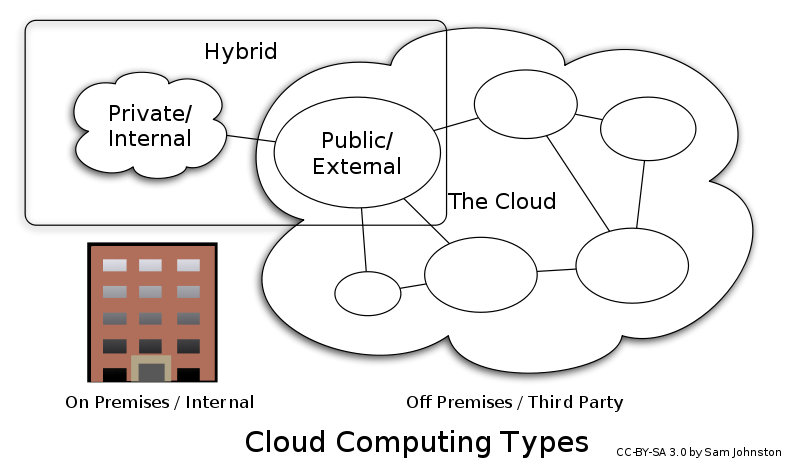
\includegraphics[width=6cm, height=4cm]{./images/dep.png}
% \end{center}
\subsection{Work in the Clouds}


Cloud computing can help with large-scale computing requirements or can lead consolidation efforts 
by virtualizing servers to make more use of existing hardware (and possibly release old hardware from service.) 
People also use cloud computing for collaboration because of the high availability through networked computers. 
Productivity suites for word processing, number crunching, and email communications, and more are also available through cloud computing.
 Cloud computing also avails additional storage to the cloud user, 
avoiding the need for additional hard drives on your desktop and enabling access to large data storage capacity online in the cloud.
 
\subsection{Conclusion}
\paragraph{} In this section we present the cloud computing in general and the differing layer which composes.
 In the two sections that follow this one, 
we will present the different cloud computing solutions and platforms of different smart phone 
and of course our choice we will adopt for our final project year.\par


%%%%%%%%%%%%%%%%%%%%%%%%%%%%%%%%%%%%%%%%%%%%%%%%%%%%%%%%%%%%%%%%%%%%%%%%%%%%%%%%%%%%%%%%%%%%%%%%%%%%%%%%%%%%%%%%%%%%%%%%%%%%%%%%%%%%%%%%%%%%%%%%%%%%%%%%%%%%
\newpage
\section{Platform}
\subsection{Eucalyptus:}

\begin{figure}[!h]
  \center
  
\includegraphics{./images/Eucalyptus-Logo.jpg}
  
\end{figure}

 



\subsubsection{Introduction:}


\paragraph{}Eucalyptus is a software available under GPL that helps in creating and managing a private or even a publicly accessible cloud.
 It provides an EC2 compatible cloud computing platform and S3 compatible cloud storage platform. 
Eucalyptus has become very popular and is seen as one of the key open source cloud platforms.
 Since Eucalyptus makes its services available through EC2/S3 compatible APIs, the client tools written for AWS can be used with Eucalyptus as well.
\subsubsection{Components of Eucalyptus}
A configuration based on Eucalyptus cloud is composed of five main types of components.

\paragraph{Node Controller (NC):}The NC (through the functionality of a hypervisor) controls VM activities,
 including the execution, inspection, and termination of VM instances.
\paragraph{Cluster Controller (CC):}
The CC controls the execution of virtual machines (VMs) running on the nodes and manages the virtual networking between VMs and between VMs and external users.
\paragraph{Cloud Controller (CLC):}The CLC is responsible for exposing and managing the underlying virtualized resources (machines (servers),
 network, and storage) via user-facing APIs. 
Currently, the CLC exports a well-defined industry standard API (Amazon EC2) and via a Web-based user interface.
\paragraph{Storage Controller (SC):}The SC provides block-level network storage that can be dynamically attached by VMs. 
The current implementation of the SC supports the Amazon Elastic Block Storage (EBS) semantics.
\paragraph{ Walrus Storage Controller (WS3):}WS3 provides a simple persistent storage service using API REST 4 and SOAP 5 and it's compatible with the API S3
It provides three main functions:
\begin{itemize}
 \item Storing virtual machine images.
 \item Storage of images taken in operation at one time.
 \item Store files and service using the S3 API.
\end{itemize}
In fact, WS3 can be considered as a simple file storage system.

\begin{figure}[!h]
 \center
 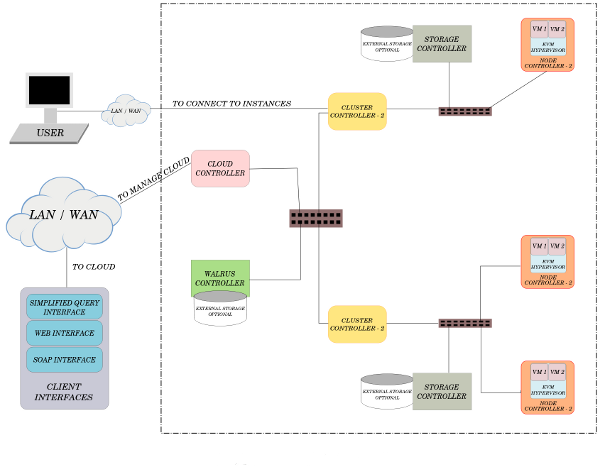
\includegraphics[width=12cm, height=9cm]{./images/ComponentsEucalyptus.png}
 \caption{Eucalyptus components}
\end{figure}



\subsubsection{Eucalyptus Software architecture:}


The Eucalyptus cloud computing platform has five high-level components: 
Cloud Controller (CLC), Cluster Controller (CC), Walrus, Storage Controller (SC) and Node Controller (NC).
 Each high-level system component has its own Web interface and is implemented as a stand-alone Web service. 
This has two major advantages: 
First, each Web service exposes a well-defined language-agnostic API in the form of a WSDL 
document containing both the operations that the service can perform and the input/output data structures.
Second, Eucalyptus leverages existing Web-service features such as security policies (WSS) for secure communication between components 
and relies on industry-standard web-services software packages.

\begin{figure}[!h]
 \center
 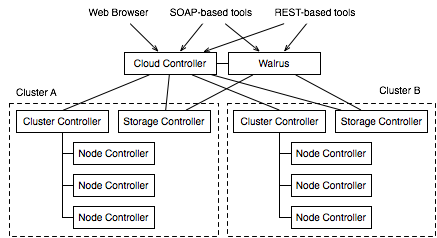
\includegraphics[width=10cm, height=5cm]{./images/EucalyptusArchitecture.png}
 \caption{Architecture Eucalyptus}
\end{figure}




In the diagram, we see that the cloud controller (CLC) and the Walrus are high-level components, with each installation in a cloud. Then the other components are divided
the various clusters that you want to use.
There are three main ways to deploy Eucalyptus:
\begin{itemize}
 \item Installing from packages.
 \item Installation from source.
 \item Installation using the Ubuntu Enterprise Cloud.
\end{itemize}
\subsubsection{Conclusion: }
Eucalyptus is a mature solution that allows the installation of a cloud infrastructure as easily as we stay in the limits of his operating.
% \subsubsection{ Prerequis:}
% \begin{onehalfspace}
% \subsubsection{The installation of the following:}
% 
% \begin{itemize}
%  \item Storage Controller (SC)
%  \item Cluster Controller (CC)
%  \item Walrus Storage Controller (WS3)
%  \item Cloud Controller (CLC)
% \end{itemize}
% 
% 
% \subsubsection{minimum hardware configuration:}
%  \begin{itemize}
%   \item CPU 1GHz
%   \item RAM 2GB
%   \item 40GB Disk Space
%   \item Hard Drive IDE 5400rpm 
%   \item  network 100Mbps
%  \end{itemize}
% 
% \subsubsection{Nodes ask for their part, the following minimum configuration:}
% \begin{itemize}
%  \item CPU VT extensions
%  \item RAM 1GB
%  \item 40GB Disk Space
%  \item Hard Drive IDE 5400rpm 
%  \item  network 100Mbps
% \end{itemize}
% 
% The key point is above the support of virtualization as it is they who will host the instances of
% virtual machines.
% \end{onehalfspace}
%------------------------------------------------------------------------------------------------------------------------------------------------------------
%%%%%%%%%%%%%%%%%%%%%%%%%%%%%%%%%%%%%%%%%%%%%%%%%%%%%%%%%%%%%%%%%%%%%%%%%%%%%%%%%%%%%%%%%%%%%%%%%%%%%%%%%%%%%%%%%%%%%%%%%%%%%%%%%%%%%%%%%%%%%%%%%%%%%%%%%%%%%
\newpage
\subsection{OpenNebula}

\begin{figure}[!h]
 \center
 
\includegraphics{./images/OpenNebula-Logo.jpg}
\end{figure}

\subsubsection{Introduction}

\paragraph{} OpenNebula is an open source project of type cloud computing IaaS. The project was launched in 2005, the first stable version was released in 2008. 
The project is licensed under Apache 2.
\paragraph{} The project aims to manage virtual machines on a large scale distributed infrastructures or cluster, and supports multiple hypervisor technologies: Xen, KVM and VMware.
OpenNebula can also combine the local and public infrastructure, which provides high modularity for hosted environments.
\paragraph{} OpenNebula is included in Debian Sid, Ubuntu and OpenSuse Natty. OpenNebula 2.2 Beta 1 was released on 02/06/2011.

\subsubsection{History}
\paragraph{}
OpenNebula was first established as a research project back in 2005 by Ignacio M. Llorente and Rubén S. Montero. 
Since its first public release of software in March 2008, it has evolved through open-source releases and now operates as an open source project.
 OpenNebula is the result of many years of research and development in efficient and scalable management of virtual machines on large-scale distributed infrastructures in close collaboration with our user community and the main cloud computing players.
 Many of its innovative features have been developed to address the requirements of business use cases from leading companies across multiple industries in the context of flagship international projects in cloud computing, such as RESERVOIR, StratusLab, BonFIRE, or 4CaaSt.
 Additionally it is being used as reference open stack for cloud computing in several large research and infrastructure projects. \par
\paragraph{}In March 2010, the main authors of OpenNebula founded C12G Labs to provide the value-added professional services that many enterprise IT shops require 
for internal adoption and to allow the OpenNebula project to not be tied exclusively to public financing,
 contributing to its long-term sustainability.
 OpenNebula.org is a project now managed by C12G Labs.\par
\begin{figure}[!h]
 \center
 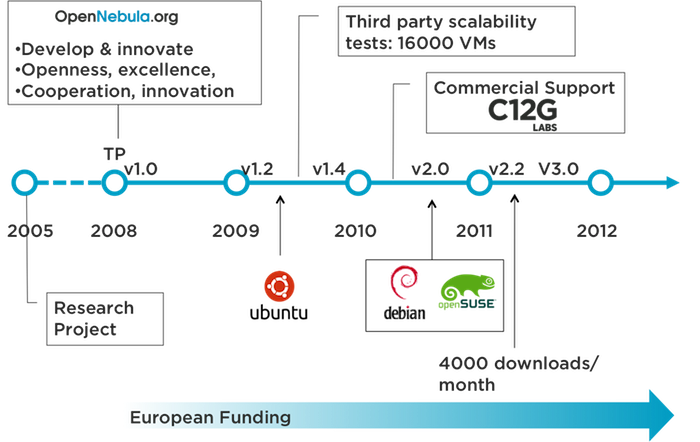
\includegraphics{./images/platform/OpenNebula/history}
\end{figure}

\subsubsection{Architecture }
\paragraph{}The OpenNebula internal architecture can be divided into three layers: 
\begin{itemize}
 \item \textbf{Tools: }management tools developed using the interfaces provided by the OpenNebula Core.
 \item \textbf{Core: }the main virtual machine, storage, virtual network and host management components.
 \item \textbf{Drivers: }to plug-in different virtualization, storage and monitoring technologies and Cloud services into the core.
\end{itemize}

\begin{figure}[!h]
\center
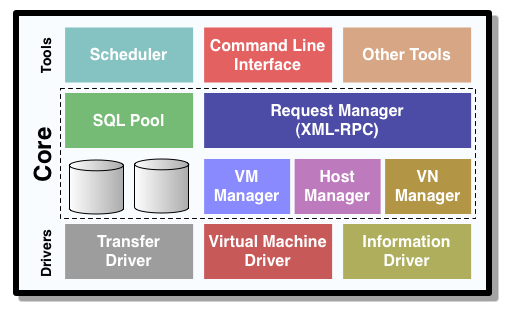
\includegraphics[height=7 cm]{./images/platform/OpenNebula/one-architecture} 
\caption{OpenNebula 2.0 Architecture }
\end{figure}

\paragraph{Tools: }
This layer contains tools distributed with OpenNebula, such as the CLI, the scheduler, the libvirt API implementation or the Cloud RESTful interfaces, and also 3rd party tools that can be easily created using the XML-RPC interface or the new OpenNebula Cloud API. 
\begin{itemize}
 \item \textbf{Command Line Interface: }A CLI for infrastructure administrators and users is provided with OpenNebula to manually manipulate the virtual infrastructure.
 \item \textbf{Scheduler: }The Scheduler is an independent entity in the OpenNebula architecture, so it can be easily tailored or changed since it is decoupled from the rest of the components. It uses the XML-RPC interface provided by OpenNebula to invoke actions on virtual machines. The scheduler distributed with OpenNebula allows the definition of several resource and load aware policies. 
\end{itemize}

\paragraph{OpenNebula Core: }The core consists of a set of components to control and monitor virtual machines, virtual networks, storage and hosts. The core performs its actions (e.g. monitor a host, or cancel a VM) by invoking a suitable driver. The main functional components of OpenNebula core are: 
\begin{itemize}
 \item \textbf{Request Manager: }to handle client requests
 \item \textbf{Virtual Machine Manager: }to manage and monitor of VMs
 \item \textbf{Transfer Manager: }to manage VM images
 \item \textbf{Virtual Network Manager: }to manage virtual networks
 \item \textbf{Host Manager: }to manage and monitor physical resources
 \item \textbf{Database: }persistent storage for ONE data structures
\end{itemize}

\paragraph{Drivers: }
OpenNebula has a set of pluggable modules to interact with specific middleware (e.g. virtualization hypervisor, cloud services, file transfer mechanisms or information services), these adaptors are called Drivers. 

\subsubsection{Conclusion:}
OpenNebula is another cloud solution, flexible and mature.
Its design is very refined, and gives great freedom to the administrator who would to deploy this solution at the cost of integration effort pushed
 to the network and other complementary solutions for storage.


%%%%%%%%%%%%%%%%%%%%%%%%%%%%%%%%%%%%%%%%%%%%%%%%%%%%%%%%%%%%%%%%%%%%%%%%%%%%%%%%%%%%%%%%%%%%%%%%%%%%%%%%%%%%%%%%%%%%%%%%%%%%%%%%%%%%%%%%%%%%%%%%%%%%%%%%%%%%%
%---------------------------------------------------------------------------------------------------------------------------------------------------------------
\newpage
\subsection{OpenStack}

\begin{figure}[!h]
 \center

\includegraphics{./images/OpenStack.png}
\end{figure}



\subsubsection{Introduction:}

 \paragraph{}OpenStack is a project from private and public cloud computing under the Apache License.
  Originally developed by NASA, the government agency which is responsible for most of the civil space program of the United States.
and Rackspace Cloud, a provider of cloud computing platform 
From July 2010, the two companies were later joined by Cloud.com, Citrix Systems,
 Dell, enStratus, NTT Data, PEER 1,RightScale, Cloudkick, Zenoss, Limelight, Scalr, AMD, Intel, Spiceworks, Canonical and Cisco for development of OpenStack.

 \paragraph{}The objective of OpenStack is to make the Cloud easy to implement and highly scalable. Ubuntu, one of the most popular Linux distributions,
 has announced that version 11.04, dubbed Natty Narwhal, will support natively OpenStack.
\newpage
\subsubsection{ Overview of Community OpenStack with Broad Commercial Support:}

\begin{figure}[!h]
 \center
 
\includegraphics[width=12cm, height=9cm]{./images/part.png}
 \caption{commercial partner OpenStack}
\end{figure}

 



\subsubsection{Components of OpenStack:}
There are currently three main components of OpenStack: Compute, Object Storage, and Imaging Service.

\paragraph{OpenStack Object Storage(Swift):}is a system to store objects in a massively scalable large capacity system with built-in redundancy and failover.
 Object Storage has a variety of applications, such as backing up or archiving data, serving graphics or videos (streaming data to a user’s browser), 
serving content with a Content Delivery Network (CDN), storing secondary or tertiary static data, developing new applications with data storage integration, 
storing data when predicting storage capacity is difficult, and creating the elasticity and flexibility of cloud-based storage for your web applications.

\paragraph{OpenStack Compute (Nova):}is a cloud fabric controller, used to start up virtual instances for either a user or a group. 
It's also used to configure networking for each instance or project that contains multiple instances for a particular project.
 
\paragraph{OpenStack Imaging Service:}is a lookup and retrieval system for virtual machine images. It can be configured in three ways: 
using OpenStack Object Store to store images; using S3 storage directly; using S3 storage with Object Store as the intermediate for S3 access.

\paragraph{Example using the three Components together: }

\begin{figure}[!h]
 \center
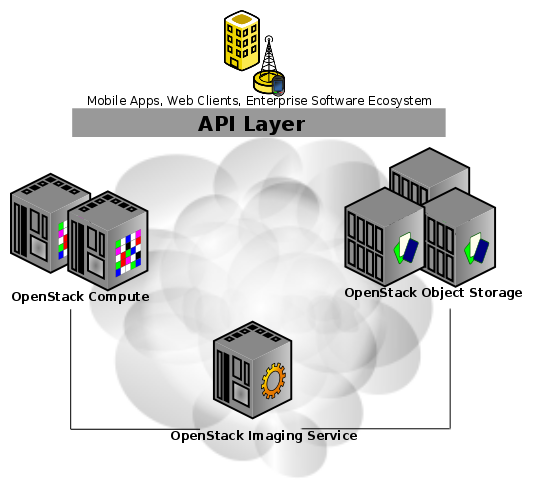
\includegraphics[width=10cm, height=8cm]{./images/OpenStackCore.png}
 \caption{Components of OpenStack}
\end{figure}





For our project we use OpenStack Compute Nova.


\subsubsection{Conclusion:}
OpenStack solution is still young but has great potential in relation to its architecture and community and the support of its partners.
 It is therefore a solution to supervise because we think it can become the reference of free cloud computing solutions.


\newpage
\subsection{Comparative table}


\begin{tabular}{|c|p{4.5cm}|p{4cm}|p{4.5cm}|}
\hline
    &Eucalytus &OpenStack &OpenNebula \\ \hline
Storage   & \textcolor{red}{very good:} A main controller walrus and storage controllers on each node.&\textcolor{red}{good:} just the basics, shared storage.&\textcolor{red}{neutral:}

by default, copy the virtual machines via SSH, managing a shared directory via NFS and ability to use a complementary solution as a distributed file system.\\ \hline
Hyperviseur    &Xen, KVM	&Xen, KVM	&Xen, KVM,VMware\\ \hline
Network    &\textcolor{red}{limited:}not designed for deployment on a complex network.&	&\textcolor{red}{Advantages and disadvantages:}Automated network simple, manual via a complex network\\ \hline
orientation    &private Cloud &public Cloud  &private Cloud \\ \hline
% security    &\textcolor{red}{good:} chaque contrôleur est authentifié par clé SSH et fichiers de permission pour authentifier toutes les transactions.	&\textcolor{red}{limited:}Très bien, authentification utilisateur par clé, utilisation des Euca2ools.&Neutre, prévu pour des utilisateurs de connance (besoin d'accès au frontend pour l'administration via libvirt ou les commandes one*)\\ \hline
install    &\textcolor{red}{problematic:}depends on the network environment and hardware problems in a heterogeneous environment.&\textcolor{red}{easy:}automated installation and documented.	&\textcolor{red}{Manual:}easy installation on the supported distributions (including Debian and Ubuntu).\\ \hline
%Maturité    &		&	&		\\ \hline
Documentation    &\textcolor{red}{correct:}complete but not always up to date.&\textcolor{red}{very good:}site well supplied and easy to access with the same time a wiki containing  the essential and an official documentation.	&\textcolor{red}{perfect:}documentation, references of all configuration files, examples. Lack of assistance in on a complex environment.		\\ \hline
%Extensibilite    &		&	&		\\ \hline
%Flexibilite    &		&	&		\\ \hline

\end{tabular}
\newpage
% \begin{onehalfspace}
% \paragraph{Eucalyptus:} is a mature solution that allows to install an infrastructure cloud quite easily  as long as we remain 
% in the subject operating. However, the purpose of cloud computing is to facilitate this evolution,Eucalyptus doesn't do that.
%   So that's why it is now abandoned for other solutions.
% \paragraph{OpenNebula:} is another solution cloud, flexible and mature. Its design is very sleek,
%  et laisse une grande liberté à l'administrateur qui souhaiterait déployer cette solution au prix d'un exort d'intégration poussé 
% au réseau et à d'autres solutions complémentaires pour le stockage. Dans cette optique, OpenNebula est une solution adaptée à Grid 5000.
% \paragraph{OpenStack:}Is a solution still young,
% but has great potential in relation to architecture and community and the support of its partners.
% It is therefore a solution to watch because it can become the reference solutions of free cloud.
% \end{onehalfspace}
%%%%%%%%%%%%%%%%%%%%%%%%%%%%%%%%%%%%%%%%%%%%%%%%%%%%%%%%%%%%%%%%%%%%%%%%%%%%%%%%%%%%%%%%%%%%%%%%%%%%%%%%%%%%%%%%%%%%%%%%%%%%%%%%%%%%%%%%%%%%%%%%%%%%%%%%%%%
\subsection{Justification:}
\paragraph{}We think OpenStack is the best solution of cloud computing. 
OpenStack Compute (nova) is open source software designed to provision and manage large networks of virtual machines, 
creating a redundant and scalable cloud computing platform. 
It gives you the software, control panels, 
and APIs required to orchestrate a cloud, including running instances, managing networks, and controlling access through users and projects. 
OpenStack Compute strives to be both hardware and hypervisor agnostic,
 currently supporting a variety of standard hardware configurations and seven major hypervisors.
\subsubsection{ OpenStack Nova Compute:}
\subsubsection{ Prerequis:}%%%%% a voir le truc de subsubsub
\paragraph{Hardware :} OpenStack components are designed to run on standard hardware.
\paragraph{Operating System:} OpenStack currently runs on Ubuntu, 
the version to use for large deployments is, preferably, Ubuntu 10.04 LTS. The community members have tested to install OpenStack
Nova on RHEL and CentOS, They have documented their approaches on the wiki OpenStack. For these other distributions GNU / Linux, 
installation on CentOS 6 seems the most viable solution because it does not suffer from dependency problems.

\paragraph{networks:} A flow rate of 1000 Mbps is suggested.

\paragraph{Data Base :}For OpenStack Compute, we can install whether  MySQL or PostgreSQL
database during the installation process of OpenStack Compute.

\subsubsection{System Architecture:}

Nova consists of seven main components, with the Cloud Controller component representing the global state and interacting with all other components.

\begin{figure}[!h]
 \center
 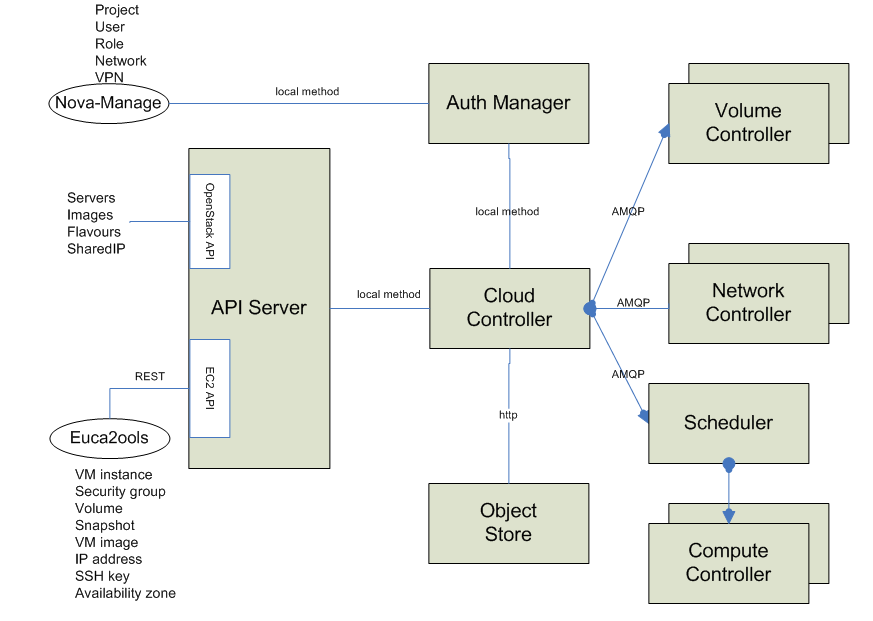
\includegraphics[width=12cm, height=10cm]{./images/arch.png}
 \caption{System Architecture}
\end{figure}


\subsubsection{Components of nova:}
\paragraph{}
Nova’s Cloud Fabric is composed of the following major components:
\begin{itemize}
 \item API Server
 \item Message Queue
 \item Compute Worker
 \item Network Controller
 \item Volume Worker
 \item Scheduler
 \item Image Store
\end{itemize}

\begin{figure}[!h]
 \center
 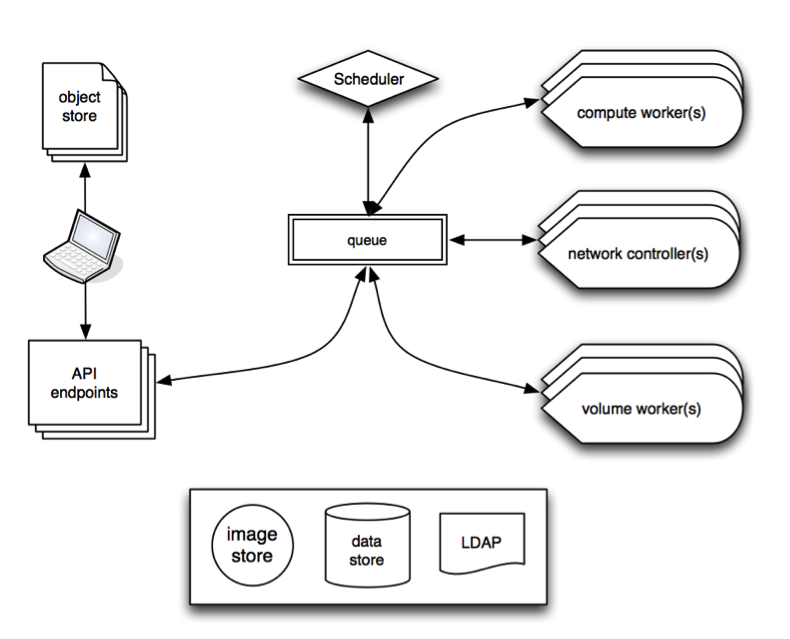
\includegraphics[width=12cm, height=10cm]{./images/components.png}
 \caption{Service Architecture}
\end{figure}



\paragraph{nova-api (API server):}At the heart of the cloud framework is an API Server. This API Server makes command and control of the hypervisor,
 storage, and networking programmatically available to users in realization of the definition of cloud computing.
\paragraph{rabbit-mq:}A messaging queue brokers the interaction between compute nodes (processing), volumes (block storage),
 the networking controllers (software which controls network infrastructure), 
API endpoints, the scheduler (determines which physical hardware to allocate to a virtual resource), and similar components.
\paragraph{nova-compute:}Compute workers manage computing instances on host machines. Through the API, commands are dispatched to compute workers to:
\begin{itemize}
 \item Run instances
 \item Terminate instances
 \item Reboot instances
 \item Attach volumes
 \item Detach volumes
 \item Get console output
\end{itemize}

\paragraph{nova-network:}The Network Controller manages the networking resources on host machines. The API server dispatches commands through the message queue, 
which are subsequently processed by Network Controllers. Specific operations include:
\begin {itemize}
 \item Allocate Fixed IP Addresses
 \item Configuring VLANs for projects
 \item Configuring networks for compute nodes
\end {itemize}

\paragraph{nova-volume:}Volume Workers interact with iSCSI storage to manage LVM-based instance volumes. Specific functions include:
\begin {itemize}
 \item Create Volumes
 \item Delete Volumes
 \item Establish Compute volumes
\end {itemize}
\paragraph{nova-scheduler:}It runs as a daemon (nova-schedule) and selects a compute / network / server volume in a pool of resources according to the algorithm 
in place. A scheduler makes decisions based on several parameters such as load, memory, cpi, or the distance to the availability zone, etc..
The Nova Scheduler implements a pluggable architecture. The algorithms available today are:
\begin{itemize}
 \item \textbf{chance:} the choice is made randomly across availability zones.
 \item \textbf{availability zone:} similar to the previous algorithm, except that the election is made in an availability zone.
 \item \textbf{simple:} This method selects the least loaded host to run the instance.
\end{itemize}
\newpage
\subsubsection{Current and future versions of Nova Compute:}

\begin{figure}[!h]
\center 
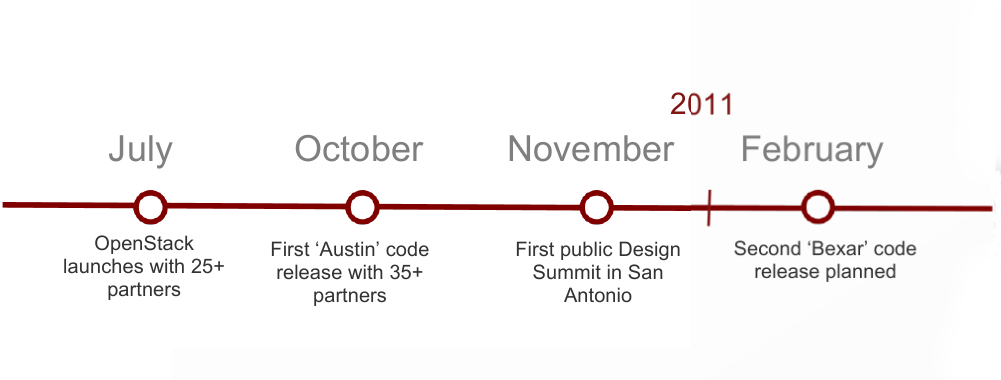
\includegraphics[width=13cm, height=6cm]{./images/history.png}
 \caption{Version of Nova Compute}

\end{figure}
%%%%%%%%%%%%%%%%%%%%%%%%%%%%%%%%%%%%%%%%%%%%%%%%%%%%%%%%%%%%%%%%%%%%%%%%%%%%%%%%%%%%%%%%%%%%%%%%%%%%%%%%%%%%%%%%%%%%%%%%%%%%%%%%%%%%%%%%%%%%%%%%%%%%%%%%%%%
\subsection{Conclusion: }
\paragraph{} Although OpenStack is a cloud solution rather young compared to other solutions described in the previous section. 
We will choose the latter, because  it's embrace of openness with both open standards and open source code.
But the important reason is it's including a large community and we don't forget the project OpenStack is considered that the solution of the future maybe,
  because it is supported by two big organizations in the world of research: Rackspace Hosting (hosting firm has broad US) and NASA (the US Space agency).\par

%%%%%%%%%%%%%%%%%%%%%%%%%%%%%%%%%%%%%%%%%%%%%%%%%%%%%%%%%%%%%%%%%%%%%%%%%%%%%%%%%%%%%%%%%%%%%%%%%%%%%%%%%%%%%%%%%%%%%%%%%%%%%%%%%%%%%%%%%%%%%%%%%%%%%%
						%Choosing the platform of the Project
%%%%%%%%%%%%%%%%%%%%%%%%%%%%%%%%%%%%%%%%%%%%%%%%%%%%%%%%%%%%%%%%%%%%%%%%%%%%%%%%%%%%%%%%%%%%%%%%%%%%%%%%%%%%%%%%%%%%%%%%%%%%%%%%%%%%%%%%%%%%%%%%%%%%%%
\newpage
\section{Platform of Smartphones}
\paragraph{}
The smartphone market is now dominated by four large companies are Apple, RIM, Google, Microsoft
 and Nokia respectively that develop operating systems iOS, Blackberry OS,
Android and Windows Phone 7 . In this section we will briefly introduce each of the systems have their advantages and disadvantages 
to know the leader in the smartphone market and determine the system that can meet most needs of the application.
%%%%%%%%%%%%%%%%%%%%%%%%%%%%%%%%%%%%%%%%%%%%%%%%%%%%%%%%%%%%%%%%%%%%%%%%%%%%%%%%%%%%%%%%%%%%%%%%%%%%%%%%%%%%%%%%%%%%%%%%%%%%%%%%%%%%%%%%%%%%%%%%%%%%%%%%%%%
\subsection{BlackBerry}

\paragraph{}
BlackBerry was created by Research In Motion (RIM), a Canadian company. It is a very popular platform especially in North America. 
A report from Gartner, the market in the U.S., the BlackBerry has maintained the No
 1 ranking with 42 percent walk. But this platform only works on BlackBerry devices.
The BlackBerry is a wireless mobile device that includes applications for smartphone apart from his cell phone capability.
 He is known for its ability to send e-mails where he has access to networks without any son of some mobile operators.
Below you find the main advantages and disadvantages of the Blackberry:
\paragraph{Advantages:}
\begin{itemize}
 \item \textbf{Security: }The Blackberry OS is the best operating system in terms of safety, it is particularly suitable for professionals.
 \item \textbf{Energy consumption: }The Smartphone developed by RIM, also,
 the advantage of consuming less energy other Smartphones competitors but also to have a superior network.
\end{itemize}
\paragraph{Disadvantages:}
\begin{itemize}
 \item \textbf{A Fee system: }One of the weaknesses of the Blackberry OS is probably the absence of Open Source that limits what applications can be used.
Indeed, Java is available on Blackberry unlike Adobe Flash. In addition, updates of the operating system to become pay beyond a number of applications.
\end{itemize}
%%%%%%%%%%%%%%%%%%%%%%%%%%%%%%%%%%%%%%%%%%%%%%%%%%%%%%%%%%%%%%%%%%%%%%%%%%%%%%%%%%%%%%%%%%%%%%%%%%%%%%%%%%%%%%%%%%%%%%%%%%%%%%%%%%%%%%%%%%%%%%%%%%%%%%%%%%
\subsection{Windows phone}
\paragraph{}
Windows Phone is a mobile operating system released in the United States October 10, 2010 and in Europe October 20, 2011. 
It is developed by Microsoft as the successor 
to the Windows Mobile platform that represents the mobile version of Microsoft Windows for mobile devices such as Smartphones or Pocket PC.
the last one is the improved version of Windows Mobile 6.5, it is for the general public rather than the business market.With Windows Phone 7, 
Microsoft offers a new user interface called Metro,which enables integration of applications in the interface further with
Hubs, icons vary depending on the situation.
\paragraph{Advantages:}
\begin{itemize}
 \item \textbf{User Interface: }Multilingual interface very clean and smoothness with nice visual effects.
 \item \textbf{The Support of the giant Microsoft: }Windows phone 7 has a Support for Microsoft, an excellent integration of Office Mobile, integration of social media and integration of "cloud" (Skydrive, Windows Live, Xbox Live) without forgetting the wireless synchronization.
\end{itemize}

\paragraph{Disadvantages: }
\begin{itemize}
 \item \textbf{Absence of several basic features: }The last baby at Microsoft has some weaknesses such as no integrated file manager, a video call, the player DivX, Xvid and Flash player. In addition, it has few third party applications and to this day is not multitasking. On the other hand, it does not allow copy / paste or file transfer via Bluetooth and the USB mass storage.
\end{itemize}


%%%%%%%%%%%%%%%%%%%%%%%%%%%%%%%%%%%%%%%%%%%%%%%%%%%%%%%%%%%%%%%%%%%%%%%%%%%%%%%%%%%%%%%%%%%%%%%%%%%%%%%%%%%%%%%%%%%%%%%%%%%%%%%%%%%%%%%%%%%%%%%%%%%%%%%%%%
\subsection{iOS}
\paragraph{}
iOS formerly iPhone OS, is the mobile operating system developed by Apple for iPhone, iPod touch and the iPad. It is derived from Mac OS X operating system from the famous Macintoshes) which it shares foundations.
\paragraph{Advantages:}
\begin{itemize}
 \item \textbf{Ergonomics: }The interface and general ergonomics of IOS reflects perfectly image of Apple: simple but elegant.
 \item \textbf{Ease of use: }Getting started is facilitated due to an intuitive management of the operating system icons and perfectly clear and easy to identify. In addition, IOS can be updated regularly.
\end{itemize}
\paragraph{Disadvantages:}
\begin{itemize}
 \item \textbf{Proprietary system: }The main weakness of IOS and products of the trademark
Apple usually resides in the fact that many of features can be used only between the same reference IPhone. For example, the user can transfer a file via Bluetooth, on his IPhone, only in other IPhone of the same generation as his..
 \item \textbf{The cost: } like all Apple products, this Smartphone running the IOS operating system is more expensive than other competing products.
\end{itemize}



%%%%%%%%%%%%%%%%%%%%%%%%%%%%%%%%%%%%%%%%%%%%%%%%%%%%%%%%%%%%%%%%%%%%%%%%%%%%%%%%%%%%%%%%%%%%%%%%%%%%%%%%%%%%%%%%%%%%%%%%%%%%%%%%%%%%%%%%%%%%%%%%%%%%%%%%%%
\subsection{Android}
\paragraph{} Android was developed by the Open Handset Alliance. Android was announced in 2007. In addition, in 2008, he became an open-source platform.
 According to Google, which is a major distributor, Android platform is a powerful, modern, safe and open. We can say Android is a complete platform for smartphones, PDAs and mobile devices. it is
composed of an operating system, libraries 'middleware' and many most applications emphasizing Google's services such as Google
Search, Google Maps or Gmail ...
Android is based on the Linux kernel, the libraries 'middleware' which composes are written
C / C + + and Java in the Framework.
\paragraph{Advantages: }
According to the latest studies and statistics done on Android, Google offers the Most upgradeable system and promising several advantages.
 The most important ones:
\begin{itemize}
 \item \textbf{Open Source: }Android supplies a free development kit (SDK) that allows to develop applications on that platform.
 \item \textbf{Language development:} which is the Java, There are many Java developers, so many people can develop for Android.
	    \begin{itemize}
	     \item Either by development-based layout and graphic components (view graphic)
	     \item Either by defining XML file (vision developer).
	    \end{itemize}

 \item \textbf{Popularity: }The Android platform has a very popular and enjoys an active community.
 \item \textbf{The number of applications on Android Market: }Android At Mobile World Congress, Activations Up 250\%, Android Market Triples Its Number Of Applications.The immense growth of Android is good for developers and users alike and shows just how popular the open ecosystem has become in the mobile market.
\end{itemize}

\paragraph{Disadvantages: }
\begin{itemize}
 \item \textbf{Slow update: }The update of the system can take a long time because of the large number of manufacturers and operators. 
Each manufacturer must adjust the update to each of its models, therefore the user is forced to wait for the update its own Smartphone.
\end{itemize}

%%%%%%%%%%%%%%%%%%%%%%%%%%%%%%%%%%%%%%%%%%%%%%%%%%%%%%%%%%%%%%%%%%%%%%%%%%%%%%%%%%%%%%%%%%%%%%%%%%%%%%%%%%%%%%%%%%%%%%%%%%%%%%%%%%%%%%%%%%%%%%%%%%%%%%%%%%
\newpage
\subsection{Comparison between different platforms}

\begin{figure}[!h]
    \begin{center}
    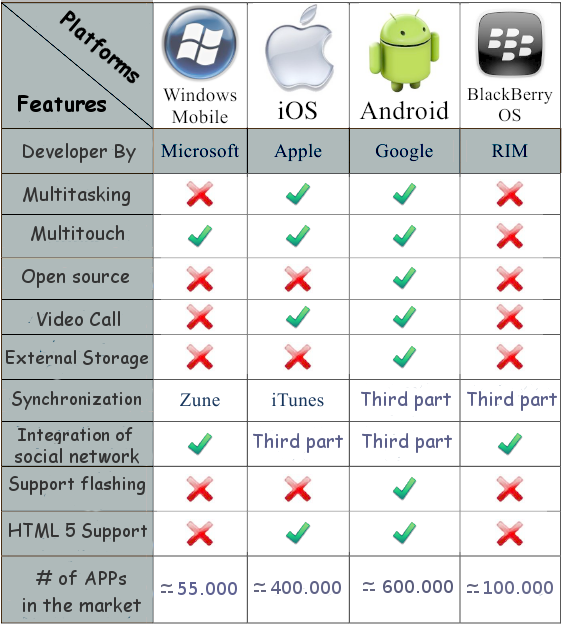
\includegraphics[width=10cm]{./images/mobile/compare}
    \caption{Superbe image}
    \end{center}

\end{figure}
%%%%%%%%%%%%%%%%%%%%%%%%%%%%%%%%%%%%%%%%%%%%%%%%%%%%%%%%%%%%%%%%%%%%%%%%%%%%%%%%%%%%%%%%%%%%%%%%%%%%%%%%%%%%%%%%%%%%%%%%%%%%%%%%%%%%%%%%%%%%%%%%%%%%%%%%%%%
\subsection{Justification:}

\paragraph{What's Android ?}

Android is a software stack for mobile devices that includes an operating system, middleware and key applications. The Android SDK provides the tools
and APIs necessary to begin developing application on the Android platform using the java programming language.
\paragraph{Features:}
\begin{itemize}
 \item \textbf{Application framework: }enabling reuse and replacement of components
 \item \textbf{Dalvik virtual machine: }optimized for mobile devices
 \item \textbf{Optimized graphics: }powered by a custom 2D graphics library; 3D graphics based on the OpenGl ES 1.0 specification (hardware acceleration optional)
engine
\item \textbf{SQLite: }for structured data storage
\item \textbf{GSM Telephony: }hardware depenndent 
\item \textbf{Media support: }for common audio,video, and still imafe formats (MPEG4, H.264, MP3, AAC, AMR, JPG, PNG, GIF)
\item \textbf{Bluetouth, EDGE,3G, and WI-FI: }hardware dependent
\item \textbf{Camera, GPS, compass, and accelerometer: }hardware dependent
\item \textbf{Rich development environment: }including a device emulator, tools for debugging, memory and performance profiling, and a plugin for the Eclipse
IDE
\item \textbf{Android Architecture: }The following diagram shows the major components of the Android operating system. Each section is described in more detail below
\begin{figure}[!h]
 \center
 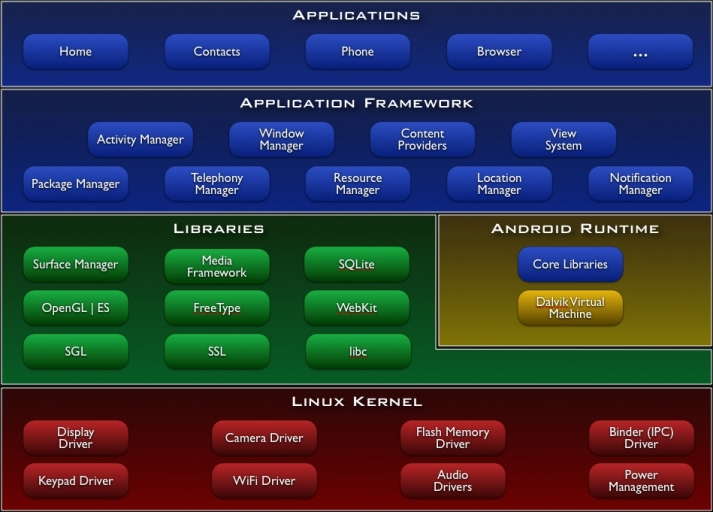
\includegraphics[width=12cm, height=10cm]{./images/mobile/arch}
 \caption{Androide Architecture}
\end{figure}
 
 \begin{enumerate}
   \item \textbf{Applications: } Android will ship a set of core applications including an email client, SMS program, calendar, maps, browser, contacts,
and others. All applications are written using the java programming language.
   \item \textbf{Applications Framework: }By providing an open development platform, Android offers developers the ability
to build extremely rich and innovative applications. Developers are free to take advantage of the device hardware, access location information, run background
services, set alarms, add notifications to the status bar, and much, much more. Developers have full access to the same framework APIs used by the core applications.
The application architecture is designed to simplify the reuse of components; any application can publish its capabilities and any other application may then 
make use of those capabilities (subject to security constraints enforced by the framework). This same mechanism allows components to be replaced by the user.
\paragraph{} Underlying all application is a set of services and systems, including:
    \begin{itemize}
	  \item A rich and extensible set of Views that can be used to build an application, including lists, grids, text boxes, buttons, and even an embeddable web
	  browser
	  \item Content Providers that enable applications to access data from other applications (such as Contacts), or to share their own data
	  \item A resource Manager, providing access ton non-code ressources such as localized strings, graphics, and layout files
	  \item A Notification Manager that enables all applications to display custom alerts in the status bar
	  \item An Activity Manager that manages the lifecycle of applications and provides a common navigation backstack
	  
    \end{itemize}

\item \textbf{Libraries in Android:}
Android includes a set of C/C++ libraries used by various components of the Android system. These capabilities are exposed to developers through the Android application
framework. Some of the core libraries are listed below:
    \begin{itemize}
     \item System C library-a BSD-derived implementation of the standard C system library(libc), tuned for embedded Linux-based devices
     \item Media Libraries- based on PacketVideo's OpenCore; the libraries support playback and recording of many popular audio and video formats, as well as
static image files, including MPEG4, H.264, MP3, AAC,AMR, JPG, and PNG
     \item Surface Manager- manages access to the display subsystem and seamlessly composites 2D and 3D graphic layers from multiple applications
     \item LibWebCore- a modern web browser engine which powers both the Android browser and an embeddable web view
     \item SGL-the underlying 2D graphics engine
     \item 3D libraries- an implementation based on OpenGL ES 1.0 APIs; the libraries use either hardware 3D acceleration (where available) or the included,
highly optimized 3D software rasterizer 
     \item FreeType-bitmap and vector font rendering 
     \item SQLite- a powerful and lightweight relational database engine available to all applications
    \end{itemize}

\item \textbf{Android Runtime:}
      \paragraph{}Android includes a set of core libraries thet provides most of the provides most of the functionality available in the core libraries of 
the java programming language.
      \paragraph{}Every Android application runs in its own process, with its own instance of the Dalvik virtual machine. Dalvik has been written so that
a device can run multiple VMs efficiently. The Dalvik VM executes files in the Dalvik Executable (.dex) format which is optimized for minimal memory footprint.
The VM is register-based, and runs classes compiled by a java language compiler that have been transformed into the .dex format by the included ``dx'' tool.
      \paragraph{}The Davlik VM relies on the Linux Kernel for underlying functionality such as threading and low-level memory management.

  \end{enumerate}


\end{itemize}
%%%%%%%%%%%%%%%%%%%%%%%%%%%%%%%%%%%%%%%%%%%%%%%%%%%%%%%%%%%%%%%%%%%%%%%%%%%%%%%%%%%%%%%%%%%%%%%%%%%%%%%%%%%%%%%%%%%%%%%%%%%%%%%%%%%%%%%%%%%%%%%%%%%%%%%%%%%
\subsection{Conclusion: }
\paragraph{} In the smartphone market almost all major brands of Mobile have released one or more models of android phone,, brands like Samsung or HTC.
Android was chosen because (almost) everything is free start with the SDK that includes an emulator (which reproduces the exact behavior of the phone) is
 a free unlike other platform and we also offer many possibilities equal or superior to another platform.\par
% utiliser include permet d'inserer des pdfs
  \chapter{Installing Nova}
\lettrine[lines=3]{W}{} ith the basics and theory behind us, it is time to get hands-on with Nova and install the code on a server. 
In this chapter, we will walk through the installation and configuration of Nova on a single node with CentOS 6.2 packages.
\section{Single Node Install}
 \paragraph{} CentOS 6.2 is available for i386 and x86\_64, as a DVD-assembly (4.6 Gb),
 the image of minimum installation (285 MB) and the reduced image for network installation - netinstall.iso (162 MB).
For our project end of year we used 
CentOS-6.2-i386-bin-DVD.\par

\newpage
\subsection{Installing CentOS:}
 
\begin{figure}[!h]
\center
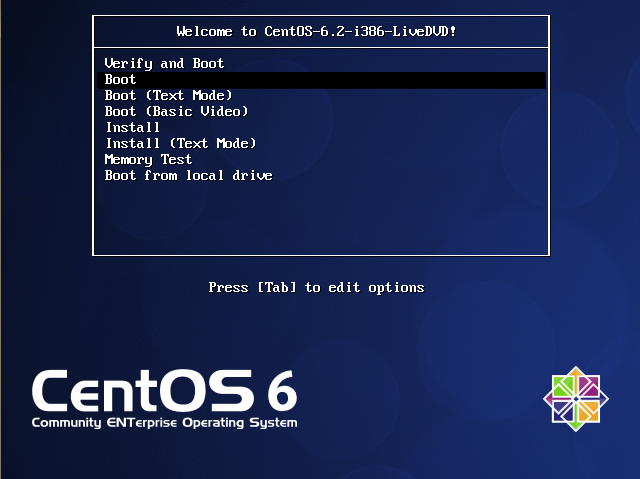
\includegraphics[width=13cm, height=8cm]{./images/install/accueil}
\caption{Installing CentOS 6.2- Home screen }
\end{figure}

\begin{figure}[!h]
 \center
 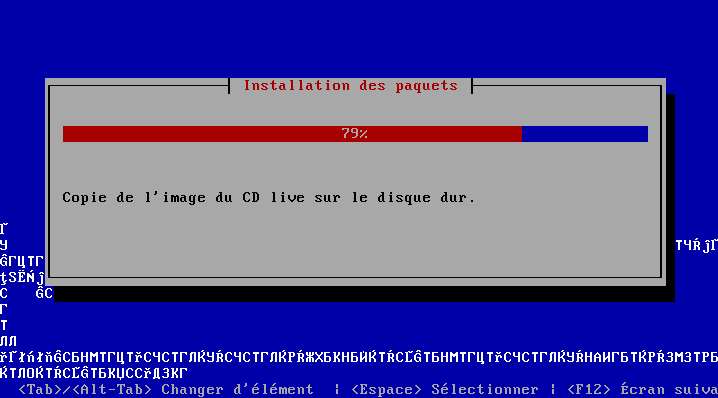
\includegraphics[width=13cm, height=8cm]{./images/install/install}
 \caption{Installing CentOs 6.2- installing packages}
\end{figure}

\newpage

\begin{figure}[!h]
 \center
 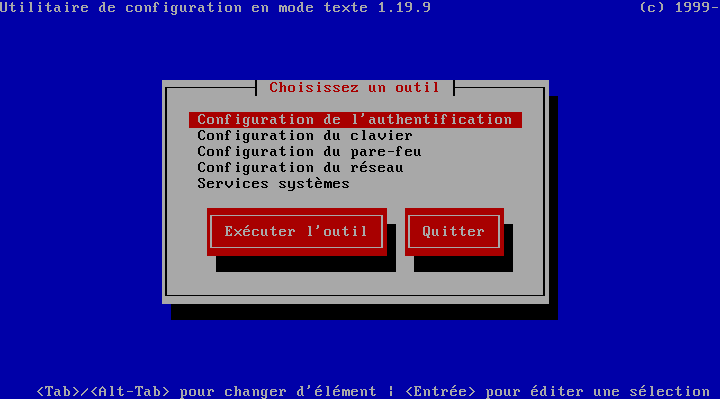
\includegraphics[width=13cm, height=9cm]{./images/install/conf}
 \caption{Installing CentOs 6.2- configuration}
\end{figure}

\begin{figure}[!h]
 \center
 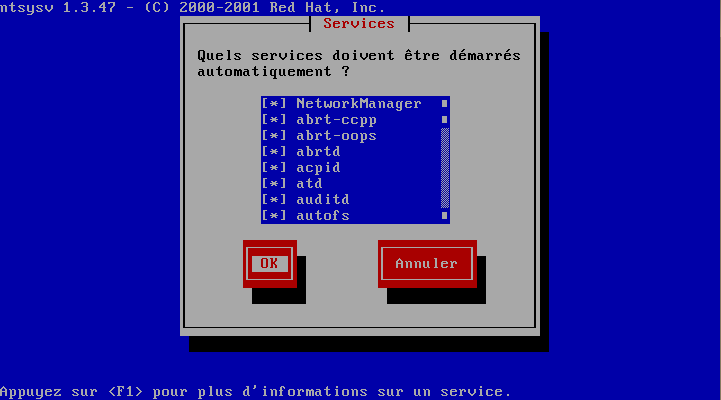
\includegraphics[width=13cm, height=9cm]{./images/install/service}
 \caption{Installing CentOs 6.2- service configuration}
\end{figure}



\newpage
\subsection{Include Repositories:}
\paragraph{}For CentOS 6.2 we need only DVD installation or an Internet connection. All dependencies included in our repository. To include our repository we create a file gd-openstack.
repo in \textbf{/etc/yum.repos.d} directory with content:


\begin{lstlisting}[language={[Latex]TeX}, numbers=left, frame=single]
[gd]
name=Packages from GridDynamics
baseurl=http://yum.griddynamics.net/yum/diablo-centos
enabled=1
gpgcheck=0
priority=1

\end{lstlisting}

And addiditionaly include EPEL and CR repositories.
\begin{lstlisting}[language={[Latex]TeX},basicstyle=\small, frame=single]
# yum install centos-release-cr
# rpm -Uvh http://download.fedora.redhat.com/pub/epel
/6/x86_64/epel-release-6-5.noarch.rpm
\end{lstlisting}

\subsection{Install nova from packages:}
\paragraph{Cloud Controller:}
We Install MySQL as oour database with the mysql-server package.\par

\begin{lstlisting}[language={[Latex]TeX}, frame=single]
# yum install mysql mysql-server
# yum install openstack-nova-node-full
# yum install euca2ools
# yum install python-novaclient
# yum install MySQL-python

\end{lstlisting}

\paragraph{}All other packages will be installed as dependencies automatically.

\subsection{Create MySQL database on Cloud Controller:}
\paragraph{}Nova uses MySQL to store information about running VMs (PostgreSQL is also possible to use).


\begin{lstlisting}[language={[Latex]TeX}, frame=single]
# mysqladmin -uroot -p -f drop nova
# mysqladmin -uroot -p create nova
\end{lstlisting}
With the database created, we now need to make an account for the user nova. We’ll just use some quick SQL statements to grant privileges 
and set the password before we login to make sure we did it correctly.We used this script (we run it without arguments) to prepare our database for nova:

\begin{lstlisting}[language={[Latex]TeX}, numbers=left, frame=single]
#!/bin/bash

DB_NAME=nova
DB_USER=nova
DB_PASS=nova
PWD=nova

HOSTS="$@"

for h in $HOSTS localhost; do
        echo "GRANT ALL PRIVILEGES ON $DB_NAME.* TO 
'$DB_USER'@'$h'IDENTIFIED BY '$DB_PASS';" | mysql -uroot -p
$PWD mysql
done
echo "GRANT ALL PRIVILEGES ON $DB_NAME.* TO $DB_USER IDENTIFIED 
BY '$DB_PASS';" | mysql -uroot -p$PWD mysql
echo "GRANT ALL PRIVILEGES ON $DB_NAME.* TO root IDENTIFIED BY
'$DB_PASS';" | mysql -uroot -p$PWD mysql

nova-manage db sync

\end{lstlisting}
\paragraph{}The nova-manage db command is rarely used except for troubleshooting and upgrades. It has two subcommands: sync and version. 
The sync subcommand will upgrade the database scheme for new versions of Nova and the version will report the current version.\par

\paragraph{}To upgrade scheme versions, use the nova-manage db sync(the last of our script). 
This should be rarely used unless we are installing from source(in our case) or upgrading our installation. 
If there are pending scheme migrations, it will apply those to your database. If there are not, it will return nothing.\par
\paragraph{}To view the database scheme version, we use the db version arguments:\par

\begin{lstlisting}[language={[Latex]TeX}, frame=single]
# nova-manage db version
\end{lstlisting}

\newpage

\subsection{Run services:}
\begin{lstlisting}[language={[Latex]TeX}, frame=single]
# service rabbitmq-server start
# service libvirtd start
# service nova-api start
# service nova-direct-api start
# service nova-compute start
# service nova-network start
# service nova-objectstore start
# service nova-scheduler start
# service glance-api start
# service glance-registry start
\end{lstlisting}
\paragraph{}Services can be monitored through the nova-manage command on a service or host basis. 
With the service, you can either view or actively manage services. For example, you can query a host for the services that it currently offers,
 or simply list all the services that are available. This is an essential command for testing or troubleshooting your deployment. 
Below is an example that walks through the full array of of service subcommands:
 listing services, enabling and disabling services, and describing resources on a host.\par



\begin{lstlisting}[language={[Latex]TeX}, frame=single]
# nova-manage service list nova-controller nova-compute
# nova-manage service disable nova-controller nova-scheduler
# nova-manage service list
# nova-manage service enable nova-controller nova-scheduler
# nova-manage service list
# nova-manage service describe_resource nova-controller

\end{lstlisting}

\paragraph{}nova-manage service also allows we to update resources that are available on a particular host. This is only applies to compute hosts.

\subsection{Configuration:}
\paragraph{}Nova administration is accomplished through a tool called nova-manage. 
Most commands take the form nova-manage command subcommand and any necessary arguments. At any time, 
you can see help for nova-manage by leaving off any arguments, subcommands, or commands.\par

\textbf{Create the network configuration:}

\begin{lstlisting}[language={[Latex]TeX}, frame=single]
# nova-manage network create novanetwork 10.0.0.0/8 1 64
\end{lstlisting}
\paragraph{}we choose fixed (private) IP address range. 
we use 10.0.0.0/8 range as long as this does not conflict with our current network settings. 
\paragraph{}For this command, the IP address is the cidr(Classless Inter-Domain Routing) notation for our netmask,
The value 1 is the total number of networks we made, and the 64 value is the number of IP addresses in each network. 

\paragraph{}Nova has a trio of nova-manage networking commands: network, fixed, and floating. The nova-manage network is the most powerful. 
It allows you to list, create, and delete networks within the Nova database.For example:\par
\paragraph{}We used this command for listing:\par

\begin{lstlisting}[language={[Latex]TeX}, frame=single]
# nova-manage network list
\end{lstlisting}

\paragraph{}The fixed command simply allows we to view the fixed IP address mappings to hostname, host, and MAC address.
esults of the command (it goes on to show the every IP address in the mapping):

\begin{lstlisting}[language={[Latex]TeX}, frame=single]
# nova-manage fixed list
\end{lstlisting}

\paragraph{}The floating command is very similar to the fixed command except that it manipulates public IP addresses.\par
%%%%%%%%%%%%%%%%%%%%%%%%%%%%%%%%%%%%%%%%%%%%%%%%%%%%Nova Administrator %%%%%%%%%%%%%%%%%%%%%%%%%%%%%%%%%%%%%%%%%%%%%%%%%%%%%%%%%%%%%%%%%%%%%%%%%%%%%%%%%%%%
\textbf{Creating User and Projects}

\paragraph{} The first step is using our new Nova installation is to create a user. 
This is a multi-step process that uses the nova-manage utility to create a project.\par
\textbf{Create a Nova administrator:}

\begin{lstlisting}[language={[Latex]TeX}, frame=single]
# nova-manage user admin nova
\end{lstlisting}
\newpage
\textbf{After that we can see an access key and a secret key export:}
\begin{lstlisting}[language={[Latex]TeX}, frame=single]
export EC2_ACCESS_KEY=e4764179-fecd-49e5-8f62-70418ffb94bb
export EC2_SECRET_KEY=9329a8c3-ad93-4176-b350-0099a43527ab
\end{lstlisting}

\textbf{Create a project for the user we created:}

\begin{lstlisting}[language={[Latex]TeX}, frame=single]
# nova-manage project create IRT nova
\end{lstlisting}

\textbf{Download credentials for ower user/project}

\begin{lstlisting}[language={[Latex]TeX}, frame=single]
# nova-manage project zipfile IRT nova
\end{lstlisting}

\textbf{Unzip and source credentials:}

\paragraph{} The final step will produce a zip-compressed file called nova.zip. Now we uncompress the credential zip file and source the resulting novarc  in ower current working directory. 
This will set a number of environmental variables needed to access your Nova installation with other utilities. 
If we are creating this user on behalf of another user, we will need to give him this zipfile.\par
\textbf{ We unzip it with this command:}
\begin{lstlisting}[language={[Latex]TeX}, frame=single]
# unzip nova.zip
\end{lstlisting}
\paragraph{}We see these files extract:\par 
\begin{lstlisting}[language={[Latex]TeX}, frame=single]
Archive:  nova.zip
 extracting: novarc
 extracting: pk.pem
 extracting: cert.pem
 extracting: nova-vpn.conf
 extracting: cacert.pem
\end{lstlisting}

%%%%%%%%%%%%%%%%%%%%%%%%%%%%%%%%%%%%%%%%%%%%%%%%%%%%%%%%%%%%%%%%%%%%%%%Register an image%%%%%%%%%%%%%%%%%%%%%%%%%%%%%%%%%%%%%%%%%%%%%%%%%%%%%%%%%%%%%%%%%%%%%
\newpage
\subsection{Register an image:}
\paragraph{}Instances are created from registered images. Before we can launch instances, we need to upload a virtual disk image into Nova. 
There are a number of different images that you can use with your Nova installation. 
You can also make your own images.\par
\textbf{Get a working image with kernal and initrd:}
\begin{lstlisting}[language={[Latex]TeX}, frame=single]
# wget http://smoser.brickies.net/ubuntu/ttylinux-uec
/ttylinux-uec-amd64-12.1_2.6.35-22_1.tar.gz
\end{lstlisting}
\begin{lstlisting}[language={[Latex]TeX}, frame=single]
# tar -xvf ttylinux-uec-amd64-12.1_2.6.35-22_1.tar.gz
\end{lstlisting}



\textbf{Bundle, upload, and register the kernel, initrd, and image}
\newline
\textbf{Kernel:}
\begin{lstlisting}[language={[Latex]TeX}, frame=single]
# euca-bundle-image -i ttylinux-uec-amd64-12.1_2.6.35-22_1-vmlinuz 
--kernel true
# euca-upload-bundle -b kernel-bucket -m /tmp
/ttylinux-uec-amd64-12.1_2.6.35-22_1-vmlinuz.manifest.xml
# euca-register kernel-bucket
/ttylinux-uec-amd64-12.1_2.6.35-22_1-vmlinuz.manifest.xml
\end{lstlisting}
\textbf{Initrd:}
\begin{lstlisting}[language={[Latex]TeX}, frame=single]
\begin{lstlisting}[language={[Latex]TeX}, frame=single]
# euca-bundle-image -i ttylinux-uec-amd64-12.1_2.6.35-22_1-initrd 
--ramdisk true
# euca-upload-bundle -b ramdisk-bucket -m /tmp
/ttylinux-uec-amd64-12.1_2.6.35-22_1-initrd.manifest.xml
# euca-register ramdisk-bucket
/ttylinux-uec-amd64-12.1_2.6.35-22_1-initrd.manifest.xml
\end{lstlisting}

\newpage

\textbf{Image:}
\begin{lstlisting}[language={[Latex]TeX}, frame=single]
# euca-bundle-image -i ttylinux-uec-amd64-12.1_2.6.35-22_1.img 
--kernel <aki name> --ramdisk <ari name>
# euca-upload-bundle -b image-bucket -m /tmp
/ttylinux-uec-amd64-12.1_2.6.35-22_1.img.manifest.xml
# euca-register image-bucket
/ttylinux-uec-amd64-12.1_2.6.35-22_1.img.manifest.xml
\end{lstlisting}

\textbf{Add a key :}

\begin{lstlisting}[language={[Latex]TeX}, frame=single]
# euca-add-keypair mykey > mykey.pem
\end{lstlisting}

\textbf{Run the vm }

\begin{lstlisting}[language={[Latex]TeX}, frame=single]
# euca-run-instances -k mykey ami-00000003
\end{lstlisting}

\paragraph{}Our instance has been launched and it is currently in the 'scheduling' state. 
If we wait a few minutes and everything goes well, it should progress to the 'running' state.
 We can check on its progress through the EC2 API with the euca-describe-instances command:

\begin{lstlisting}[language={[Latex]TeX}, frame=single]
# euca-describe-instances
\end{lstlisting}

\paragraph{}We can also use the nova utility to make the same query through the OpenStack API. With this tool, you are looking for the 'ACTIVE' status:\par

\begin{lstlisting}[language={[Latex]TeX}, frame=single]
# nova list
\end{lstlisting}
%%%%%%%%%%%%%%%%%%%%%%%%%%%%%%%%%%%%%%%%%%%%%%%%%%%%%%%%%%%%%%%%%%%%%%%%%%%%%%%%%%%%%%%%%%%%%%%%%%%%%%%%%%%%%%%%%%%%%%%%%%%%%%%%%%%%%%%%%%%%%%%%%%%%%%%%%
\section{Conclusion: }
in this chapter, we presented the step of installing nova and some commande how to manipulate them.
  \chapter{Design Phase}
\section{Object Oriented Analysis using UML}
\begin{wrapfigure}[5]{l}{4cm}

\includegraphics[width=4cm]{./images/implementation/uml}
\end{wrapfigure}
\paragraph{}The Unified Modeling Language (UML) is a standard language for specifying, visualizing, constructing, and documenting the artifacts
 of software systems, as well as for business modeling and other non-software systems. The UML represents
a collection of the best engineering practices that have proven successful in the modeling of large and complex systems. The UML is very important parts of developing
object oriented software and the software development process. The UML uses mostly graphical notations to express the design of software projects. Using the UML
helps projects teams communicate, explore potential designs, and validate the architectural design of the software.\par
\section{Use Case}
\paragraph{}We describes in this section, the general use case diagram so this use case describes the functionality provided by a system in terms
of actors, her we have two actors user(client) and admin, their goals represented as use cases, and any dependencies among those use case.
\begin{figure}[!h]
 \center
 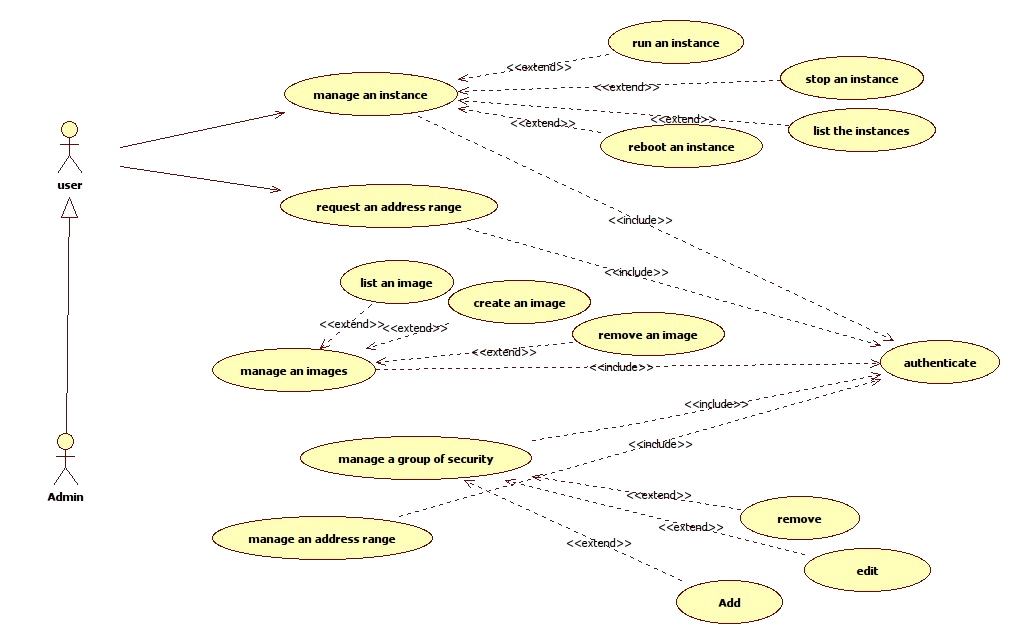
\includegraphics[width=16cm, height=12cm]{./images/design/usecase}
 \caption{Use Case Diagram}
\end{figure}

\section{Sequence diagram}
\paragraph{A sequence diagram}
\paragraph{}in a Unified Modeling Language (UML) is a kind of interaction diagram that shows how processes operate with one another and in what order. 
It is a construct of a Message Sequence Chart. A sequence diagram shows object interactions arranged in time sequence. 
It depicts the objects and classes involved in the scenario and the sequence of messages exchanged between the objects needed to carry out 
the functionality of the scenario. 
Sequence diagrams typically are associated with use case realizations in the Logical View of the system under development.\par
\paragraph{}Sequence diagrams are sometimes called event diagrams, event scenarios, and timing diagrams.\par

\begin{figure}[!h]
 \center
 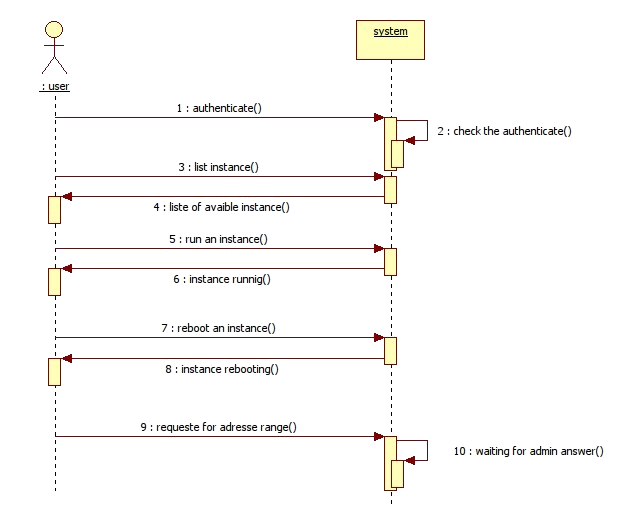
\includegraphics[width=18cm, height=15cm]{./images/design/sequenceuser}
 \caption{diagram sequance consumer}
\end{figure}

\begin{figure}[!h]
 \center
 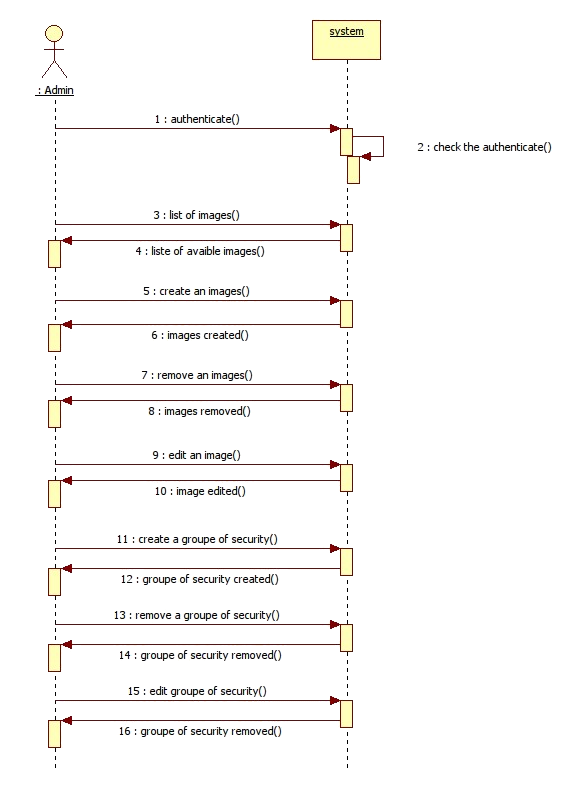
\includegraphics[width=16cm, height=19cm]{./images/design/sequenceadmin}
 \caption{diagram sequance admin}
\end{figure}

\clearpage

\section{Package Diagram}



\paragraph{}To move to the development, we rely on the principles of object-oriented approach. To this end, weare moving from a functional structure through the 
use case, to a structure object through the classes and packages. It is important to gather classes in packages to better understand the overall role of each
party and facilitate code maintenance. To identify the packages, we relied on two criteria: consistency and independence.

\begin{figure}[!h]
 \center
 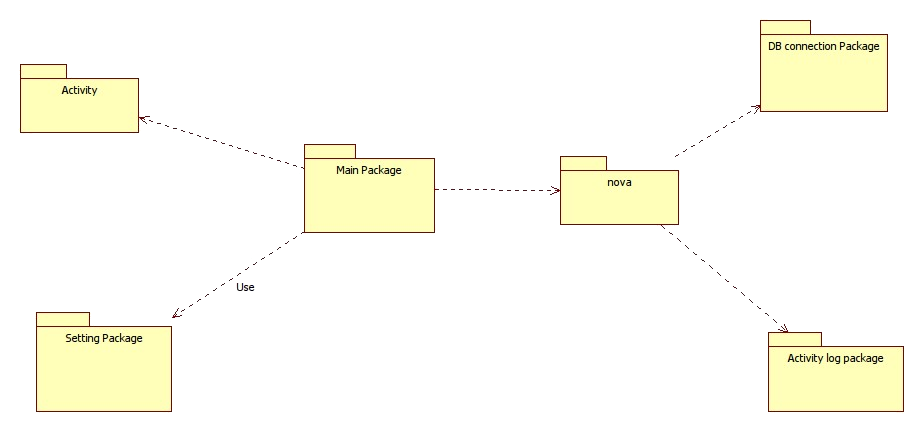
\includegraphics[width=12cm, height=10cm]{./images/design/package}
 \caption{diagram sequance admin}
\end{figure}
% \section{Class Diagram }
% \paragraph{}The class diagram is a static diagram. It represents the static view of an application.Class diagram
% is not only used for visualizing, describing and documenting different aspects of a system but also for constructing executable code of
% the software application. It describes the attributes and operations of a class and also the constraints imposed on the system, the class
% diagrams are widely used in the modeling of object oriented systems because they are the only UML diagrams which can be mapped directly with object oriented
% languages. The Class diagram pf our application is shown in the following figure.\par
\newpage
\section{Deployment Diagram}
\paragraph{}the deployment diagram shows the physical arrangement of materials that make up the distribution system and components of these materials.\par
\paragraph{}hardware resources are represented as nodes and these nodes are connected together by means of a communication medium.\par
\begin{figure}[!h]
 \center
 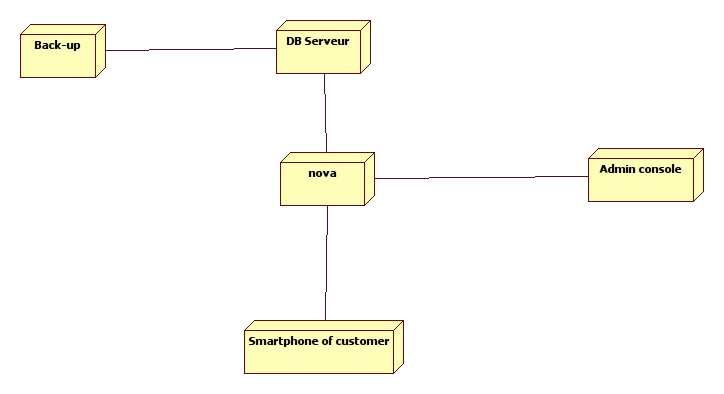
\includegraphics[width=12cm, height=8cm]{./images/design/deployment}
 \caption{Use Case Diagram}
\end{figure}

\section{Conclusion}
\paragraph{}
In the design phase the architecture was established, the different classes of the application are now classified, it is time for implementing our 
application
  \chapter{Implementation and testing}
\lettrine[lines=3]{T}{} he last part of this document will describe the implementation process of the application we are developing. In the first paragraph
we will specify our development environment: Hardware, systems, developing tools and frame works, the second paragraph will be reserved for the application's
screen shots
\section{Hardware environment}
\begin{wrapfigure}[4]{r}{3cm}
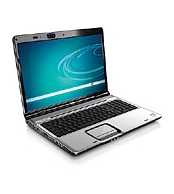
\includegraphics[width=4cm]{./images/implementation/me}
\end{wrapfigure}
\textbf{Server:} 
HP Pavilion dv9865ek Entertainment Notebook PC\newline
Intel core 2 Duo processor T8300\newline
2.4 GHZ, level 2 cache 3 MB\newline
3072 MB (1 X 1024 MB + 1 X 2048)\newline
500 GB (2X250 GB) SATA Hard Disk Drive 5400 rpm\\
\newpage
\begin{wrapfigure}[4]{r}{3cm}
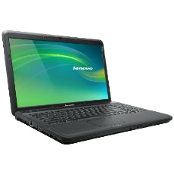
\includegraphics[width=4cm]{./images/implementation/you}
\end{wrapfigure}

\textbf{Client:}
 LENOVO G550 NTD8FFR\newline
 Intel core 2 Duo processor T6570\newline
 2.10 GHZ, level 2 cache 3 MB\newline
 3072 MB (1 X 1024 MB + 1 X 2048)\newline
 320 GB  SATA Hard Disk Drive 5400 rpm\newline
\section{Operating system}
This application was developed on Gnu/Linux system and it will be run in the mobile operating system called Android.


\section{Developing Tools}
\subsection{Eclipse}
\begin{wrapfigure}[4]{r}{3cm}

\includegraphics[width=4cm]{./images/implementation/Eclipselogo}
\end{wrapfigure}
\paragraph{Eclipse}is an integrated development environment free extensible, universal and versatile,allowing to create development projects implementing any programming language.
IDE Eclipse is written mainly in Java (using the graphics library SWT, IBM), and this language, through specific library, is also used to write extensions.
\paragraph{}The specification of Eclipse comes from the fact of its architecture fully developed around the concept of plug-in (in accordance with the OSGi standard):
the functionality of this software workshop are developed as plug-in.
\paragraph{}Several commercial software are based on free software, such as IBM Lotus Notes 8, Symphony or IBM WebSphere Studio Application Developer.
\paragraph{}This integrated development environment is a freeware set of tools to develop software in one (or more) language (s) programming. Eclipse is:
\begin{itemize}
 \item \textbf{A specialized text editor}(with syntax highlighting, automatic indentation, auto completion, ...),
 \item \textbf{A compiler}(or at least the integration of an existing compiler),
 \item \textbf{A debugger}(or at least the integration of an existing debugger)
 \item \textbf{A set of tools}for automating the compilation and management projects,
\end{itemize}
\subsection{StarUML:}
\begin{wrapfigure}[4]{r}{3cm}

\includegraphics[width=4cm]{./images/implementation/StarUML}
\end{wrapfigure}
\paragraph{}was an open source UML tool, licensed under a modified version of GNU GPL. After being abandoned for some time, 
the project had a last revival to move from Delphi to Java/Eclipse and stop again. However, 
the community is still active and many topics are discussed on the forums.\par
\paragraph{}The stated goal of the project was to replace larger, commercial applications such as Rational Rose and Borland's Together.\par
\paragraph{}StarUML supports most of the diagram types specified in UML 2.0. It is currently missing object, package, 
timing and interaction overview diagrams (though the first two can be adequately modeled through the class diagram editor).\par

\paragraph{} StarUML was written in Delphi, which is one of the reasons[1] why it was abandoned for a long time.\par

\subsection{Gimp}
\begin{wrapfigure}[4]{r}{3cm}

\includegraphics[width=4cm]{./images/implementation/gimp}
\end{wrapfigure}
\paragraph{Gimp}
is a free and open source software raster graphics editor. It is primarily employed as an image retouching and editing tool
and is freely available in versions tailored for most popular operating systems including Microsoft Windows, Apple Mac OS X, and Linux.\par
\paragraph{}
In addition to detailed image retouching and free-form drawing, GIMP can accomplish essential image editing tasks such as resizing,
 editing, and cropping photos, photomontages combining multiple images, and converting between different image formats.
 GIMP can also be used to create animated images in many formats such as GIF and MPEG through the Animation Plugin.\par
\paragraph{}
GIMP's product vision is that GIMP is a free software high-end graphics application for the editing and creation of original images, icons, graphical elements of web pages and art for user interface elements.
\subsection{Latex}
\begin{wrapfigure}[4]{l}{4cm}

\includegraphics[width=4cm]{./images/implementation/latex}
\end{wrapfigure}
\paragraph{Latex: } is a document markup language and document preparation system for the TeX typesetting program. 
Within the typesetting system, its name is styled as LaTeX. The term LaTeX refers only to the language in which documents are written, 
not to the editor used to write those documents. In order to create a document in LaTeX, a .tex file must be created using some form of text editor. 
While most text editors can be used to create a LaTeX document, 
a number of editors have been created specifically for working with LaTeX.\par 
\paragraph{}As it is distributed under the terms of the LaTeX Project Public License (LPPL), LaTeX is free software.\par
\subsection{JSON}
\begin{wrapfigure}[4]{l}{4cm}

\includegraphics[width=4cm]{./images/implementation/json}
\end{wrapfigure}
\paragraph{JSON: }(Java Object Notation) is a lightweight text-based open standard designed for human-readable data interchange.
 It is derived from the JavaScript scripting language for representing simple data structures and associative arrays, 
called objects. Despite its relationship to JavaScript, it is language-independent, with parsers available for many languages.\par

\paragraph{}The JSON format was originally specified by Douglas Crockford, and is described in RFC 4627. 
The official Internet media type for JSON is application/json. The JSON filename extension is \textbf{.json}.
\paragraph{}The JSON format is often used for serializing and transmitting structured data over a network connection.
 It is used primarily to transmit data between a server and web application, serving as an alternative to XML.\par
\subsection{JAVA}
\begin{wrapfigure}[5]{l}{4cm}

\includegraphics[width=4cm]{./images/implementation/java}
\end{wrapfigure}
\paragraph{JAVA: }Java is a programming language originally developed by James Gosling at Sun Microsystems 
(which has since merged into Oracle Corporation) and released in 1995 as a core component of Sun Microsystems' Java platform.
The language derives much of its syntax from C and C++ but has a simpler object model and fewer low-level facilities. Java applications are typically 
compiled to bytecode (class file) that can run on any Java Virtual Machine (JVM) regardless of computer architecture.\par
\paragraph{}The original and reference implementation Java compilers, virtual machines, and class libraries were developed by Sun from 1995. As of May 2007, 
in compliance with the specifications of the Java Community Process, 
Sun relicensed most of its Java technologies under the GNU General Public License. 
Others have also developed alternative implementations of these Sun technologies, such as the GNU Compiler for Java and GNU Classpath.\par
\section{realization: }
\paragraph{} The result of our application is the different interfaces to present to users.
The application is a downloadable and can be installed on different mobile devices that work
on Android operating systems.

\begin{figure}[!h]
 \center
 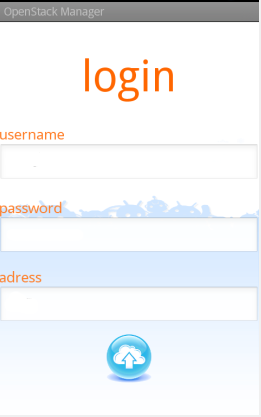
\includegraphics[width=6cm, height=8cm]{./images/implementation/login}
 \caption{connection interface}
\end{figure}
\paragraph{}This interface is the first interface that appears to the user as soon as he starts the application. 
This interface is the connection interface where the user puts his his login, 
password and address cloud.

\begin{figure}[!h]
 \center
 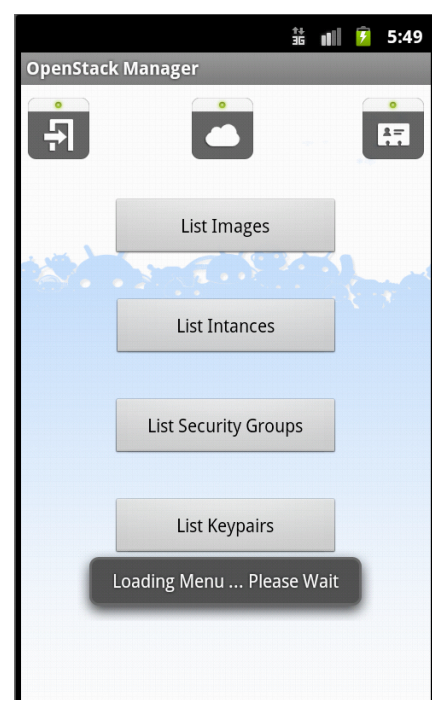
\includegraphics[width=6cm, height=8cm]{./images/implementation/menu}
 \caption{Menu List}
\end{figure}
\paragraph{}
In this second capture that is the menu list. This menu contains the different list of the application of available images,  the list of instances created, 
list of security group the user belongs etc...


\begin{figure}[!h]
 \center
 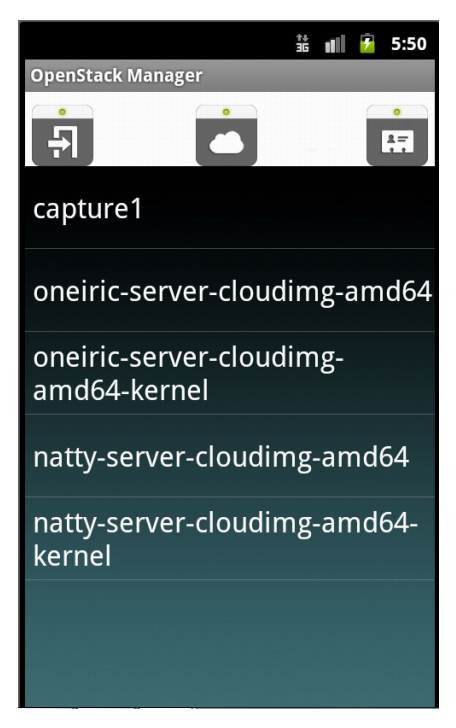
\includegraphics[width=6cm, height=8cm]{./images/implementation/images}
 \caption{Menu List}
\end{figure}
\paragraph{}in this  capture we see the difference images we have in our cloud. With this different Image API, we can create an instance by the Compute API
\section{Conclusion: }
\paragraph{}In this chapter we presented the work environment and the required tools of our application.
We have also detailed the different realization steps of the project by showing the different
interfaces of our application.\par

  \chapter{General Conclusion:}
\lettrine[lines=3]{A}{} t the end of our course of ower study, we were asked to complete a final project year. 
Our work is based on the development of a program on Mobile (Smartphone) that can manage a cloud. 
This led us to discover a new development platform and enrich our knowledge and experience in cloud computing.
\paragraph{}Indeed, this project was to achieve a mobile application combining the features of using  cloud computing and a mobile phone needs. 
This accomplishment made us spend enough time especially in terms of research, 
development and testing of several options where we had difficulties.
\paragraph{}These challenges overcome, helped to enrich ourselves by forging technical skills prerequisite and
 we learn to overcome the technical difficulties. 
To anticipate future changes we want to ensure the development of our application whatsoever aside technical or architectural side.
\paragraph{}The realization of this project during our year-end project has served us well in the
as it led us to discover about the programming of mobile applications, deploiyement a cloud computing and of course to fix any problems that reveal their designs.

  \backmatter%netbiographie
  \chapter{Netographie}

\begin{itemize}
 
  \item https://geni-orca.renci.org/trac/wiki/OpenStack-Install
  \item http://www.griddynamics.com/openstack/setup\_single.html
 \item http://wiki.openstack.org/NovaInstall/CentOSNotes
 \item http://wiki.openstack.org/NovaInstall/DevPkgInstall
 \item http://nova.openstack.org/2011.2/
 \item http://developer.android.com/sdk/index.html
 \item http://wiki.frandroid.com\/wiki/Accueil
 \item https://trystack.org/
\end{itemize}

  
% \end{onehalfspace}
%---------------------------------------------------------------------------------------------------------
\end{document}
